\documentclass[conference]{IEEEtran}
\IEEEoverridecommandlockouts
% The preceding line is only needed to identify funding in the first footnote. If that is unneeded, please comment it out.
\usepackage{cite}
\usepackage{amsmath,amssymb,amsfonts}
\usepackage{algorithmic}
\usepackage{graphicx}
\usepackage{textcomp}
\usepackage{xcolor}
\def\BibTeX{{\rm B\kern-.05em{\sc i\kern-.025em b}\kern-.08em
    T\kern-.1667em\lower.7ex\hbox{E}\kern-.125emX}}
\begin{document}

\title{Dead Tree Semantic Segmentation\\
{\huge CS9517: Group Project}
}

\author{\IEEEauthorblockN{1\textsuperscript{st} Aayush Bajaj}
\IEEEauthorblockA{z5362216@ad.unsw.edu.au}
\and

\IEEEauthorblockN{2\textsuperscript{nd} Given Name Surname}
\IEEEauthorblockA{\textit{dept. name of organization (of Aff.)} \\
\textit{name of organization (of Aff.)}\\
City, Country \\
email address or ORCID}
\and
\IEEEauthorblockN{3\textsuperscript{rd} Given Name Surname}
\IEEEauthorblockA{\textit{dept. name of organization (of Aff.)} \\
\textit{name of organization (of Aff.)}\\
City, Country \\
email address or ORCID}
\and
\IEEEauthorblockN{4\textsuperscript{th} Given Name Surname}
\IEEEauthorblockA{\textit{dept. name of organization (of Aff.)} \\
\textit{name of organization (of Aff.)}\\
City, Country \\
email address or ORCID}
\and
\IEEEauthorblockN{5\textsuperscript{th} Given Name Surname}
\IEEEauthorblockA{\textit{dept. name of organization (of Aff.)} \\
\textit{name of organization (of Aff.)}\\
City, Country \\
email address or ORCID}
\and
\IEEEauthorblockN{6\textsuperscript{th} Given Name Surname}
\IEEEauthorblockA{\textit{dept. name of organization (of Aff.)} \\
\textit{name of organization (of Aff.)}\\
City, Country \\
email address or ORCID}
}

\maketitle

\begin{abstract}
    TODO
\end{abstract}

\begin{IEEEkeywords}
    semantic segmentation, cnn, unet, svm, random forests, 
\end{IEEEkeywords}

\section{Introduction}

\section{Literature Review}

\section{Methods}
\subsection{DeepLabV3\,+CBAM for Fine–Grained Semantic Segmentation}
\label{sec:seg_deeplab_cbam}
DeepLabV3+ is a semantic image segmentation model built on top of a standard CNN ``backbone" for feature extraction. Its encoder-decoder structure fuses high-level context with low-level(high resolution) features via skip connections, yielding sharp object boundaries. 
\paragraph{Motivation.}
Dead-tree pixels cover $\approx$3\,\% of each radiograph and appear as thin,
low-contrast structures.  
We therefore require \emph{(i)} large receptive fields to recognise context
and \emph{(ii)} high spatial fidelity to preserve edges.  
DeepLabV3 supplies the former via
Atrous Spatial Pyramid Pooling (ASPP), while
CBAM supplies the latter by letting the network
\textit{focus} on informative channels and regions.

\paragraph{Pre-processing.}
Images are resized to \(256\times256\), stacked into six channels
(R, G, B, NIR, G, B), then per-channel $z$-score normalised.
All images are first resized to \(256 \times 256\) so that the network sees a
\emph{fixed} spatial grid; this eliminates per-image padding, keeps the
receptive-field schedule constant, and enables efficient, size-homogeneous
mini–batching on the GPU.
Including NIR enriches the spectral signature: vegetation stress and
water content modulate NIR much more strongly than the visible bands, and
duplicating \(G,B\) lets early convolutions learn cross-spectral filters
(e.g.\ “\(\text{NIR}-\text{G}\)” indices) that correlate with
dead-tissue pixels yet are tricky to hand-engineer.
Finally, each channel is $z$-score normalised,
\(x' = (x - \mu) / \sigma\),
centering the distribution at zero and scaling it to unit variance.
This removes scale disparities between bands, keeps gradients numerically
stable, and prevents high-energy channels (typically NIR) from dominating the
loss.  The combined resizing, stacking, and normalisation pipeline therefore
standardises the data, maximises useful spectral diversity, and supplies the
CNN with well-behaved inputs that converge faster and yield sharper,
more discriminative features.

\paragraph{Encoder with embedded attention.}
A lightweight \textbf{ResNet-18} backbone produces four feature stages
\(\{f_1,f_2,f_3,f_4\}\) at strides \(\{4,8,16,32\}\).
After each residual block we insert a \textbf{CBAM} to refine features.

\paragraph{Attention mechanism.}
Given \(F\in\mathbb{R}^{C\times H\times W}\), channel and spatial masks are
computed as
\begin{align}
  M_c &= \sigma\!\bigl(
           W_1\,\mathrm{GAP}(F)+
           W_2\,\mathrm{GMP}(F)
         \bigr),\\
  \hat F &= M_c \odot F,\\
  M_s &= \sigma\!\Bigl(
           \mathrm{Conv}_{7\times7}
           \bigl[\mathrm{GAP}(\hat F);\mathrm{GMP}(\hat F)\bigr]
         \Bigr),\\
  F_{\text{CBAM}} &= M_s \odot \hat F,
\end{align}
where \(\sigma\) is the sigmoid, \(\odot\) denotes broadcast multiplication,
and GAP/GMP are global average/max pooling. 
\emph{Channel attention} amplifies the metal-rich filters;
\emph{spatial attention} pinpoints their contours.

\begin{figure}
  \centering
  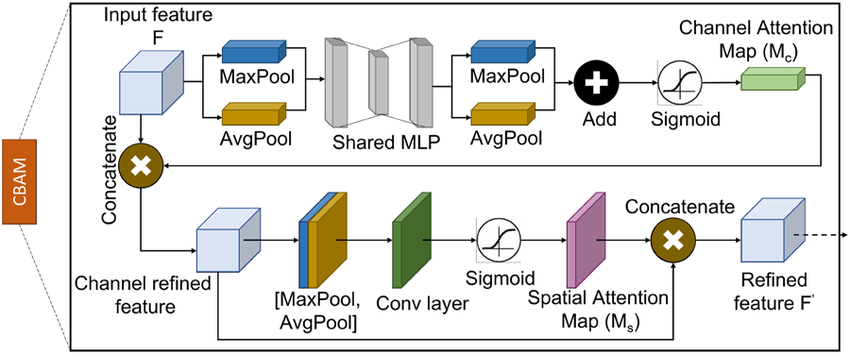
\includegraphics[width=.72\linewidth]{figs/cbam_block.png}
  \caption{CBAM: sequential \emph{channel} (\(M_c\)) and
           \emph{spatial} (\(M_s\)) attention. Adapted from}
  \label{fig:cbam}
\end{figure}

\paragraph{Atrous Spatial Pyramid Pooling.}
The top feature map \(f_4\) is processed by ASPP branches
\(\{1\times1, 3\times3_{r=6}, 3\times3_{12}, 3\times3_{18},
\text{global pool}\}\).
Concatenation (\(5\times256\) channels) is compressed to 256 channels
via a \(1\times1\) convolution.

Convolutional layers with a single dilation rate see only one scale of
context: either fine detail (small rate) or broad structure (large rate).


\begin{figure}
  \centering
  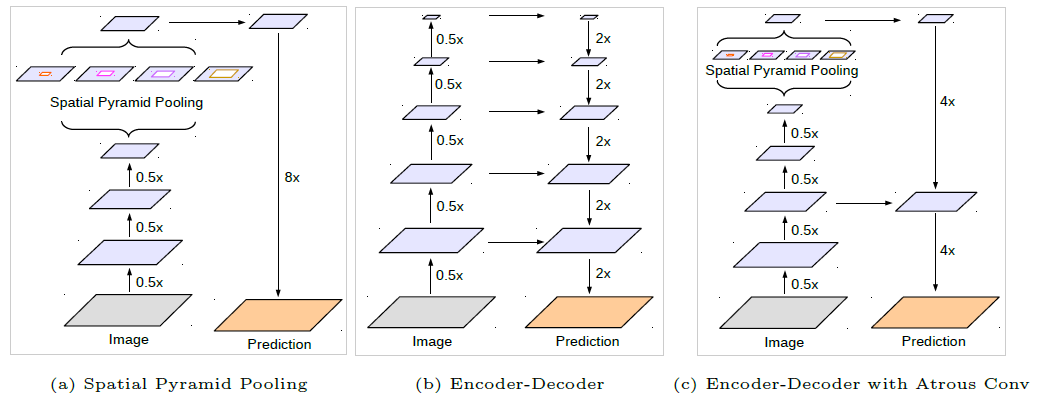
\includegraphics[width=.9\linewidth]{figs/aspp.png}
  \caption{Encoder–decoder topology of DeepLabV3\,+. Atrous rates
           \(\{1,6,12,18\}\) provide multi–scale context; a skip connection
           injects low-level detail for sharp boundaries.}
  \label{fig:deeplabv3p}
\end{figure}

\paragraph{Decoder.}
The ASPP tensor is $4\times$ bilinearly upsampled and concatenated with
\(f_1\) (stride-4).  
A single \(3\times3\) \(\rightarrow\) BN \(\rightarrow\) ReLU layer refines the
fusion; dropout \(p{=}0.3\) regularises; a \(1\times1\) convolution produces
per-pixel logits which are finally upsampled to the original resolution.

\paragraph{Loss and optimisation.}
We minimise a composite loss
\begin{equation}
  \mathcal{L} = \alpha\,\mathcal{L}_{\text{BCE}} +
                \beta\,\mathcal{L}_{\text{Dice}} +
                \gamma\,\mathcal{L}_{\text{Tversky}},
  \quad (\alpha,\beta,\gamma)=(0.3,0.3,0.4),
\end{equation}
with the Tversky term
\begin{equation}
\mathcal{L}_{\text{Tversky}}
  = 1 - \frac{\!\!\sum_i p_i g_i}
             {\sum_i p_i g_i
              + 0.3\sum_i p_i(1-g_i)
              + 0.7\sum_i (1-p_i)g_i},
\end{equation}
balancing precision and recall on minority pixels.  
Training uses AdamW (lr \(=10^{-3}\), wd \(=10^{-4}\)),
`ReduceLROnPlateau` (factor 0.5, patience = 5), batch size = 8.

Binary-cross-entropy (BCE) supplies a pixel-wise “log-likelihood’’ signal that stabilises early training: it pushes every pixel toward its correct class regardless of region size and keeps gradients dense, which helps the optimiser escape flat regions of the loss landscape. Dice loss then counters the imbalance directly by maximising the overlap ratio between prediction and ground truth; because it is normalised by the combined foreground areas, a handful of minority pixels can still exert a proportionally large influence, preventing the network from converging to a trivial all-background solution. Finally, the Tversky loss generalises Dice with separate weighting on false positives and false negatives (here we set \begin{math}\alpha = 0.3, \beta = 0.7\end{math}). That asymmetry is crucial for thin, low-contrast structures such as dead-tree branches: it penalises missed foreground (false negatives) more heavily than spurious foreground, nudging the model to “err on the side of inclusion’’ and recover slender details that Dice alone often overlooks. By linearly combining the three terms, we preserve BCE’s stable gradients, Dice’s overlap sensitivity, and Tversky’s controllable precision–recall trade-off, yielding masks that are both globally accurate and faithful to fine structures.
\subsection{CNN}
Convolutional neural networks (CNN) are often used to process image problems, such as object detection, object classification and segmentation\cite{b8}. We explored two different models to segment standing dead trees in aerial forest images. The first model used multiple convolutional layers with ReLU activation and batch normalisation. Each layer utilises 3 x 3 kernels with the same padding to maintain the spatial dimensions. Dropout layers are used to prevent overfitting. In the final layer, the sigmoid activation layer is used for binary segmentation output. This model is easier and faster to train and , but it also has limited ability to capture multi-scale spatial data. 

\begin{lstlisting}[language=Python]
#Model 1
#Build the simple CNN model without pooling
def cnn_simple_model(input_shape, filters, conv_layers, dropout):
    inputs = layers.Input(shape=input_shape)
    x = inputs
    for i in range(conv_layers):
        x = layers.Conv2D(filters[i], (3, 3), activation='relu', padding='same')(x)
        x = layers.BatchNormalization()(x)
        if dropout > 0:
            x = layers.Dropout(dropout)(x)
    outputs = layers.Conv2D(1, (1, 1), activation='sigmoid')(x)
    model = models.Model(inputs, outputs)
    return model
\end{lstlisting}

For the second model, it uses encoder and decoder to build the model. Encoder path uses max pooling for downsampling, while decoder path applies transposed convolution for upsampling to restore the spatial resolution. Skip connection is used for keeping spatial details, which can improve boundary accuracy. This model can capture more relevant information and finer details from images, while requiring higher computational resources and greater memory consumption for training and testing. 

\begin{lstlisting}[language=Python]
#Model 2
#Build the complex CNN model with encoder and decoder
def cnn_encoder_decoder_model(input_shape, filters, conv_layers, dropout):
    inputs = layers.Input(shape=input_shape)
    x = inputs
    skips = []
    #encode
    for i in range(conv_layers):
        x = layers.Conv2D(filters[i], (3, 3), activation='relu', padding='same')(x)
        x = layers.BatchNormalization()(x)
        skips.append(x)
        x = layers.MaxPooling2D((2, 2))(x)
        if dropout > 0:
            x = layers.Dropout(dropout)(x)

    #decode
    for i in range(conv_layers-1, -1, -1):
        x = layers.Conv2DTranspose(filters[i], (3, 3), strides=(2, 2), activation='relu', padding='same')(x)
        if i < len(skips):
            x = layers.Concatenate()([x, skips[i]])
        if dropout > 0:
            x = layers.Dropout(dropout)(x)

    outputs = layers.Conv2D(1, (1, 1), activation='sigmoid')(x)
    model = models.Model(inputs, outputs)
    return model
\end{lstlisting}

\subsection{Random Forests}
Random Forest methods refer to the use of a machine learning method that works by creating multiple decision trees and aggregating their output to produce a model which can produce a more robust and stable prediction model compared with using singular decision trees that have a tendency to overfit.\\
\\
\begin{figure}[bht!]
    \centering
    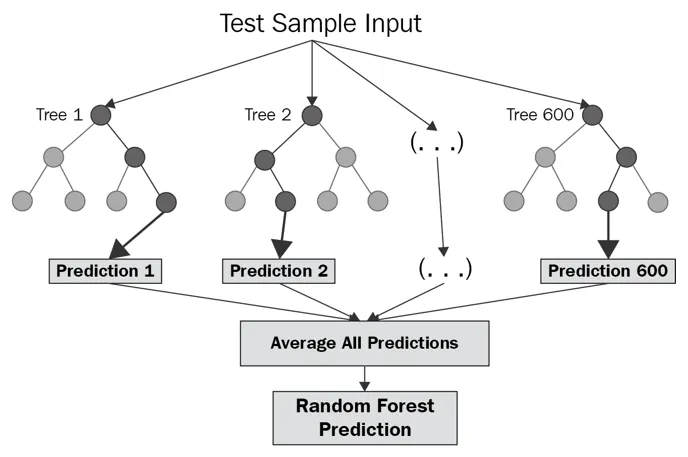
\includegraphics[width=1\linewidth]{figs/random-forest.png}
    \caption{Random forest classifier}
    \label{fig:placeholder}
\end{figure}
\\
This method was implemented in two different ways. The first method was to treat each pixel independently of the next, and only consider if the ground truth had a dead tree at that spot. This was implemented because early exploratory data analysis had noticed that dead tree pixels tended to share similar colour features compared with non-dead (regular) tree pixels.  As if the colours of the image provided a good idea if the spot contained a dead tree, it would be best not to provide too much data.\\

The second method was to consider the pixels in relation to their surroundings, as there was a chance that a dead tree would be better identified in relation to their surroundings, and in this case, taking each pixel independently would result in loss of useful data. as such the second method was to use a kernel to feed both the points and its relevant surroundings into the random forest (with the y data simply being 1 if any pixel in the kernel is a mask pixel). Since this might provide a very large data set if a kernel is made for all points, feature detection algorithms can be used to select the points, in this case, SIFT was used, but recommendations have been made for the use of other feature extraction algorithms.

\subsection{Stochastic Gradient Descent}
Another simple machine learning method that was also explored was the use of stochastic gradient descent (or SGD for short). SGD is a popular machine learning technique that applies the concept of gradient descent to minimise a loss function through iterative optimisation ~\cite{b9}.\\ Compared with traditional gradient descent where the entire training set is used in each iteration which can be very computationally expensive for large datasets ~\cite{b10}, SGD aims to alleviate this issue by choosing random samples (hence the term stochastic) . This also offers the benefit of avoiding local minima that can sometimes occur with regular gradient descent.\\ 
In the context of this project, the SGD model attempts to classify whether or not a certain vector of pixel values corresponds to a dead tree pixel or a background (non dead-tree) pixel. Similar to the random forest method, each pixel is computed independently of its surrounding neighbours (or its parent image).\\
\subsection{Support Vector Machines}
Support Vector Machines (SVM for short) is another popular supervised machine learning algorithm that aims to perform binary classification by attempting to divide a dataset using a hyperplane with a (n-1) hyperplane where n corresponds to the number of features each training sample has.\cite{b11}\\
Also known as a linear classifier, SVMs work by attempting to find a hyperplane such that the distance between the closest sample of each class is maximised. Although it is a linear classifier, SVMs are capable of performing classification even when a dataset is not linearly separable through a technique known as a kernel method or kernel trick that maps existing data into a higher dimensional space and attempting to find a suitable hyperplane in a higher dimension.~\cite{b12}\\
\\
\begin{figure}[ht]
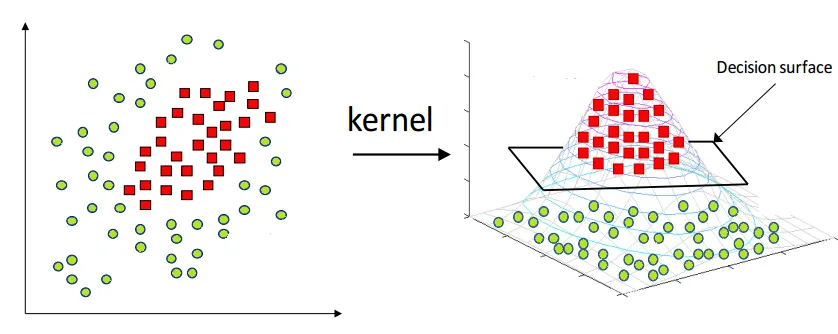
\includegraphics[width=1\linewidth]{figs/svm-kernel-trick.png}
\caption{Kernel Trick in SVM to perform linear classification on non-linearly separate data}
\label{fig:svm}
\end{figure}

However, a major downside to SVMs is if the dataset is unbalanced or noisy, resulting in classes with overlapping features. This can make it very difficult to separate different classes and if the feature space is not large enough, it may not be possible to converge on a solution as was the case with this task.\\

\subsection{UNet}
\label{sec:aj_unet}

U-Net is a fully convolutional encoder-decoder architecture originally designed for biomedical image segmentation\,\cite{b13}. Its symmetric design with skip connections enables precise boundary localisation by combining high-level semantic features with low-level spatial details. Our implementation extends the classical U-Net to leverage multi-spectral imagery and domain-specific spectral indices.\footnote{this is why we choose not to bruteforce a fantastic perfomance with \hyperlink{https://github.com/MIC-DKFZ/nnUNet}{nnUNet}; \emph{domain-knowledge}.}

\begin{figure}
  \centering
  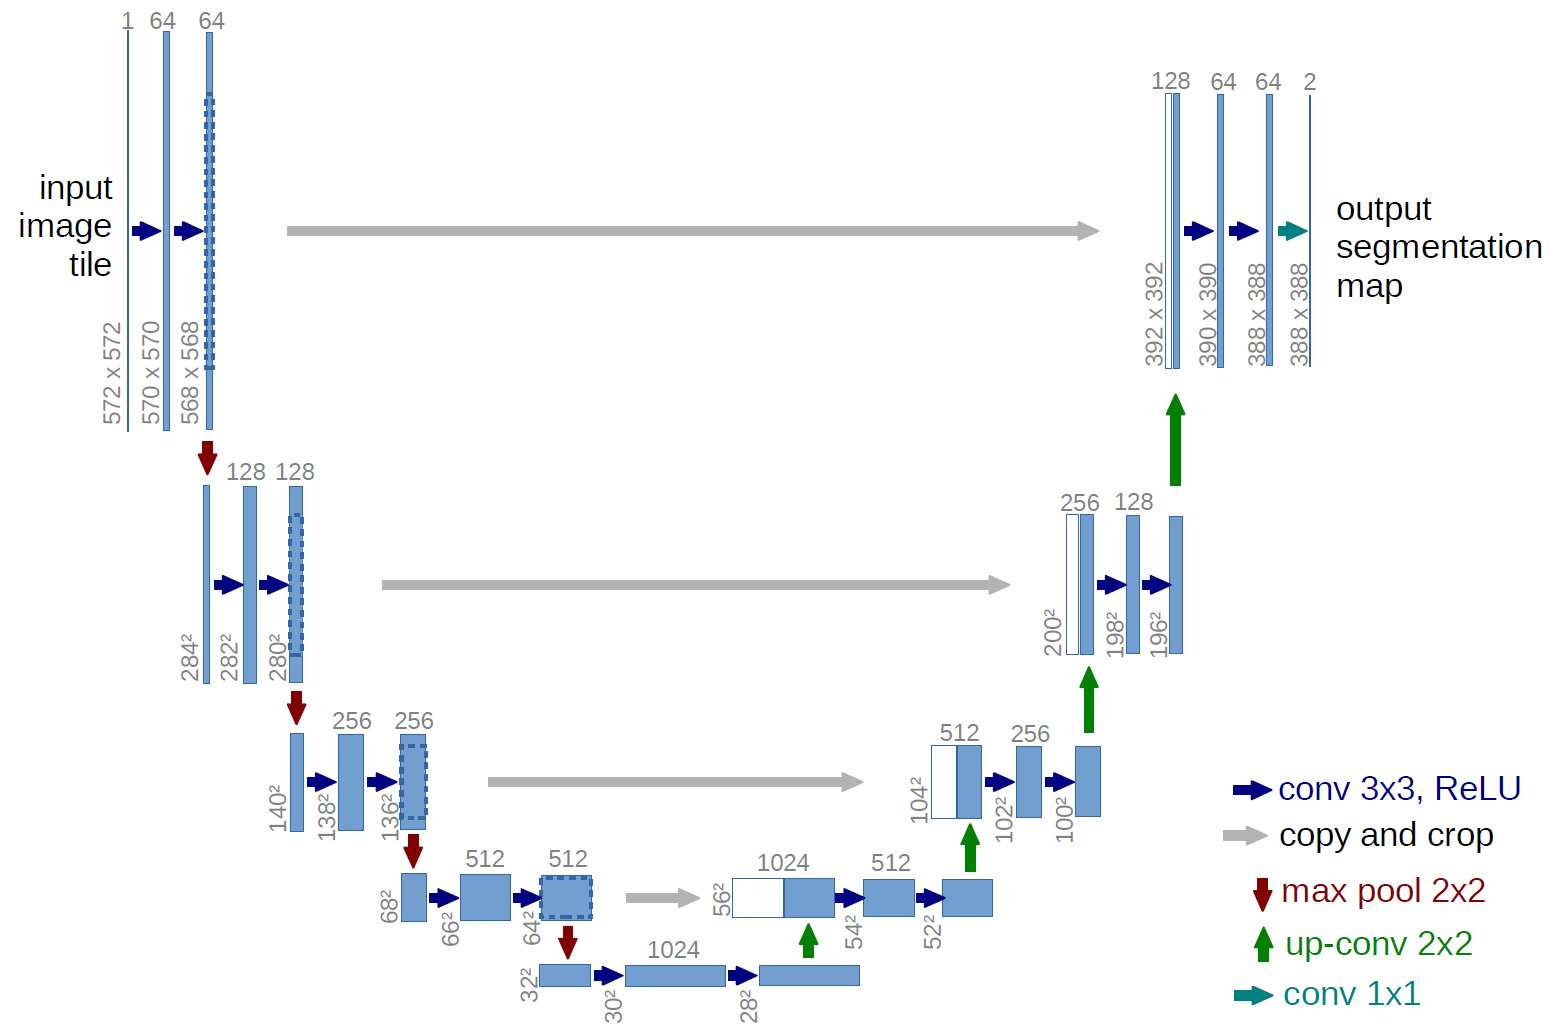
\includegraphics[width=.9\linewidth]{figs/unet-proto.jpg}
  \caption{Prototypical UNet Architecture}
  \label{fig:unet_proto}
\end{figure}

\paragraph{Motivation.}
Dead trees exhibit distinct spectral signatures across visible and near-infrared bands. Healthy vegetation reflects strongly in NIR while absorbing in red wavelengths, whereas stressed or dead vegetation shows reduced NIR reflectance. By incorporating both RGB and NRG (Near-infrared, Red, Green) channels alongside computed spectral indices, we provide the network with domain-specific features that enhance dead tree discrimination.

\paragraph{Multi-Channel Input Pipeline.}
Our dataset loader constructs 8-channel inputs by concatenating RGB channels, NRG channels, and two computed spectral indices:

\begin{lstlisting}[language=Python]
# extract individual channels for spectral indices
# RGB: R=0, G=1, B=2
# NRG: N=0, R=1, G=2 (NIR, Red, Green in NRG image)
red = rgb_tensor[0:1]      # red rgb
green = rgb_tensor[1:2]    # green rgb  
blue = rgb_tensor[2:3]     # blue rgb
nir = nrg_tensor[0:1]      # nir, nrg

# NDVI: (nir - red) / (nir + red)
eps = 1e-8 # div by 0 error
ndvi = (nir - red) / (nir + red + eps)

# ndwi = (green - nir) / (green + nir)  
ndwi = (green - nir) / (green + nir + eps)

# concatenating:
image_8ch = torch.cat([rgb_tensor, nrg_tensor, ndvi, ndwi], dim=0)  # (8, H, W)
\end{lstlisting}

The Normalised Difference Vegetation Index (NDVI)\,\cite{b14} and Normalised Difference Water Index (NDWI)\,\cite{b15} are computed as:
\begin{align}
  \text{NDVI} &= \frac{\text{NIR} - \text{Red}}{\text{NIR} + \text{Red}}, \\
  \text{NDWI} &= \frac{\text{Green} - \text{NIR}}{\text{Green} + \text{NIR}}.
\end{align}

NDVI quantifies vegetation health and photosynthetic activity, with values near +1 indicating healthy vegetation and values near -1 or 0 indicating stressed or dead vegetation. NDWI captures water stress in vegetation, providing complementary information for dead tree identification.

\begin{figure}
  \centering
  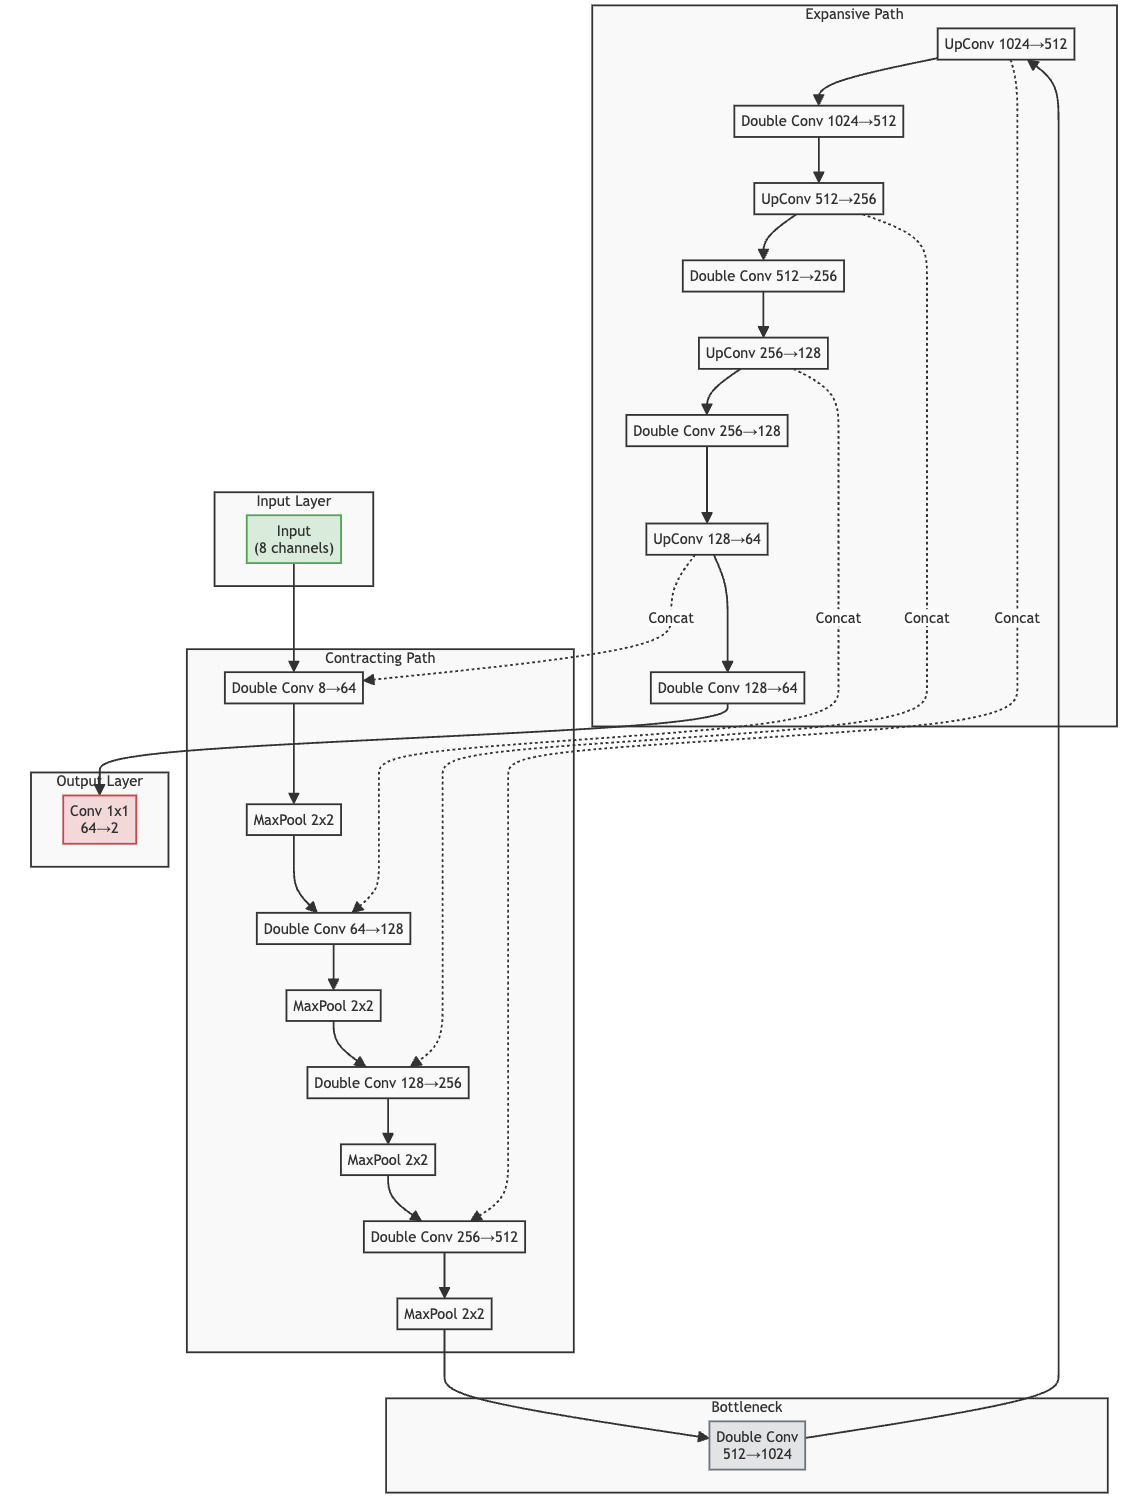
\includegraphics[width=.9\linewidth]{figs/unet-merm.jpg}
  \caption{UNet architecture: 8-channel encoder-decoder with skip connections. The contracting path captures context while the expansive path enables precise localisation. Visualisation, courtesy of torchviz \cite{b16} and Claude \cite{b17}}
  \label{fig:aj_unet_arch}
\end{figure}

\paragraph{Network Architecture.}
The U-Net encoder consists of four downsampling stages, each containing double convolutions followed by max pooling:

\begin{lstlisting}[language=Python]
class DoubleConvolution(nn.Module):
    def __init__(self, in_channels: int, out_channels: int):
        super().__init__()
        self.first = nn.Conv2d(in_channels, out_channels, kernel_size=3, padding=1)
        self.act1 = nn.ReLU()
        self.second = nn.Conv2d(out_channels, out_channels, kernel_size=3, padding=1)
        self.act2=nn.ReLU()

    def forward(self, x: torch.Tensor):
        x = self.first(x)
        x = self.act1(x)
        x = self.second(x)
        return self.act2(x)
\end{lstlisting}

The contracting path progressively reduces spatial resolution \((256^2 \rightarrow 128^2 \rightarrow 64^2 \rightarrow 32^2 \rightarrow 16^2)\) while increasing feature channels \((8 \rightarrow 64 \rightarrow 128 \rightarrow 256 \rightarrow 512 \rightarrow 1024)\). The expansive path reverses this process via transposed convolutions, concatenating corresponding encoder features through skip connections to preserve spatial information.

\paragraph{Loss Function Design.}
Class imbalance poses a significant challenge with dead trees comprising only $\approx$3\% of pixels. We address this with a composite loss combining Dice and Focal losses:

\begin{lstlisting}[language=Python]
class CombinedLoss(nn.Module):
    def __init__(self, dice_weight=0.5, focal_weight=0.5, alpha=0.25, gamma=2.0):
        super().__init__()
        self.dice_weight = dice_weight
        self.focal_weight = focal_weight
        self.dice_loss = DiceLoss()
        self.focal_loss = FocalLoss(alpha=alpha, gamma=gamma)
        
    def forward(self, outputs, targets):
        dice = self.dice_loss(outputs, targets)
        focal = self.focal_loss(outputs, targets)
        return self.dice_weight * dice + self.focal_weight * focal
\end{lstlisting}

The combined loss is:
\begin{equation}
  \mathcal{L} = \lambda_{\text{Dice}}\mathcal{L}_{\text{Dice}} + \lambda_{\text{Focal}}\mathcal{L}_{\text{Focal}},
  \quad (\lambda_{\text{Dice}}, \lambda_{\text{Focal}}) = (0.5, 0.5),
\end{equation}

where the Focal loss term addresses class imbalance:
\begin{equation}
\mathcal{L}_{\text{Focal}} = -\alpha(1-p_t)^\gamma \log(p_t),
\end{equation}
with $\alpha = 0.25$ and $\gamma = 2.0$ to down-weight easy examples and focus learning on hard cases.

\begin{figure}
  \centering
  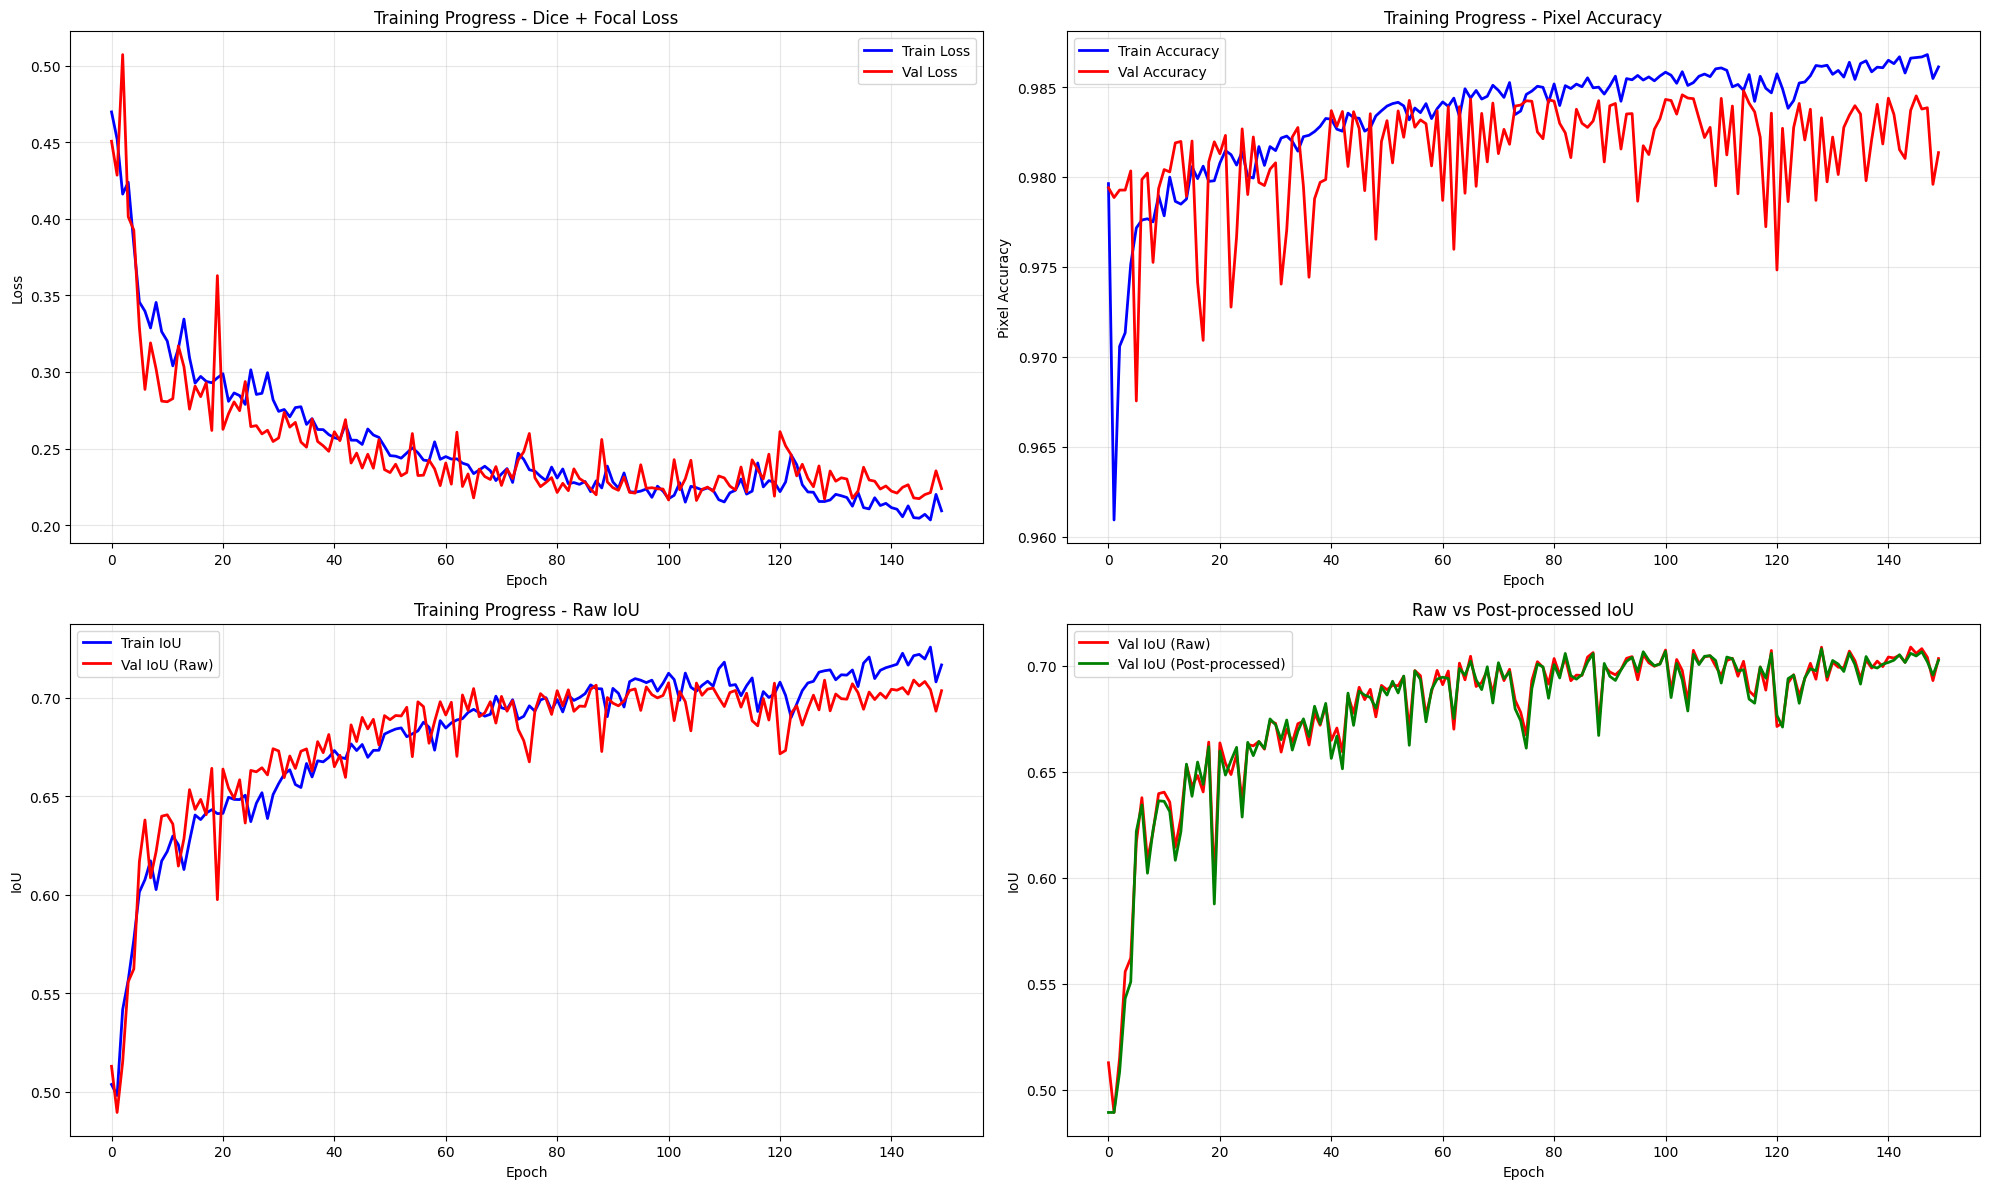
\includegraphics[width=.9\linewidth]{figs/unet-train-curve.jpg}
  \caption{Training progression showing convergence of combined Dice-Focal loss and IoU metrics over 150 epochs. Post-processing consistently improves validation IoU.}
  \label{fig:training_curves}
\end{figure}

\paragraph{Post-Processing Pipeline.}
Raw network predictions are refined through a two-stage post-processing pipeline:

\begin{enumerate}
\item \textbf{Probability Thresholding:} Dead tree probabilities are thresholded at 0.6 rather than the default 0.5, reducing false positives in ambiguous regions.
\item \textbf{Morphological Operations:} Sequential opening (erosion→dilation) removes noise, followed by closing (dilation→erosion) to fill holes in detected regions.
\end{enumerate}

This pipeline yields substantial IoU improvements ($+0.04$ typical) by cleaning spurious activations while preserving true positive detections.

\begin{figure}
  \centering
  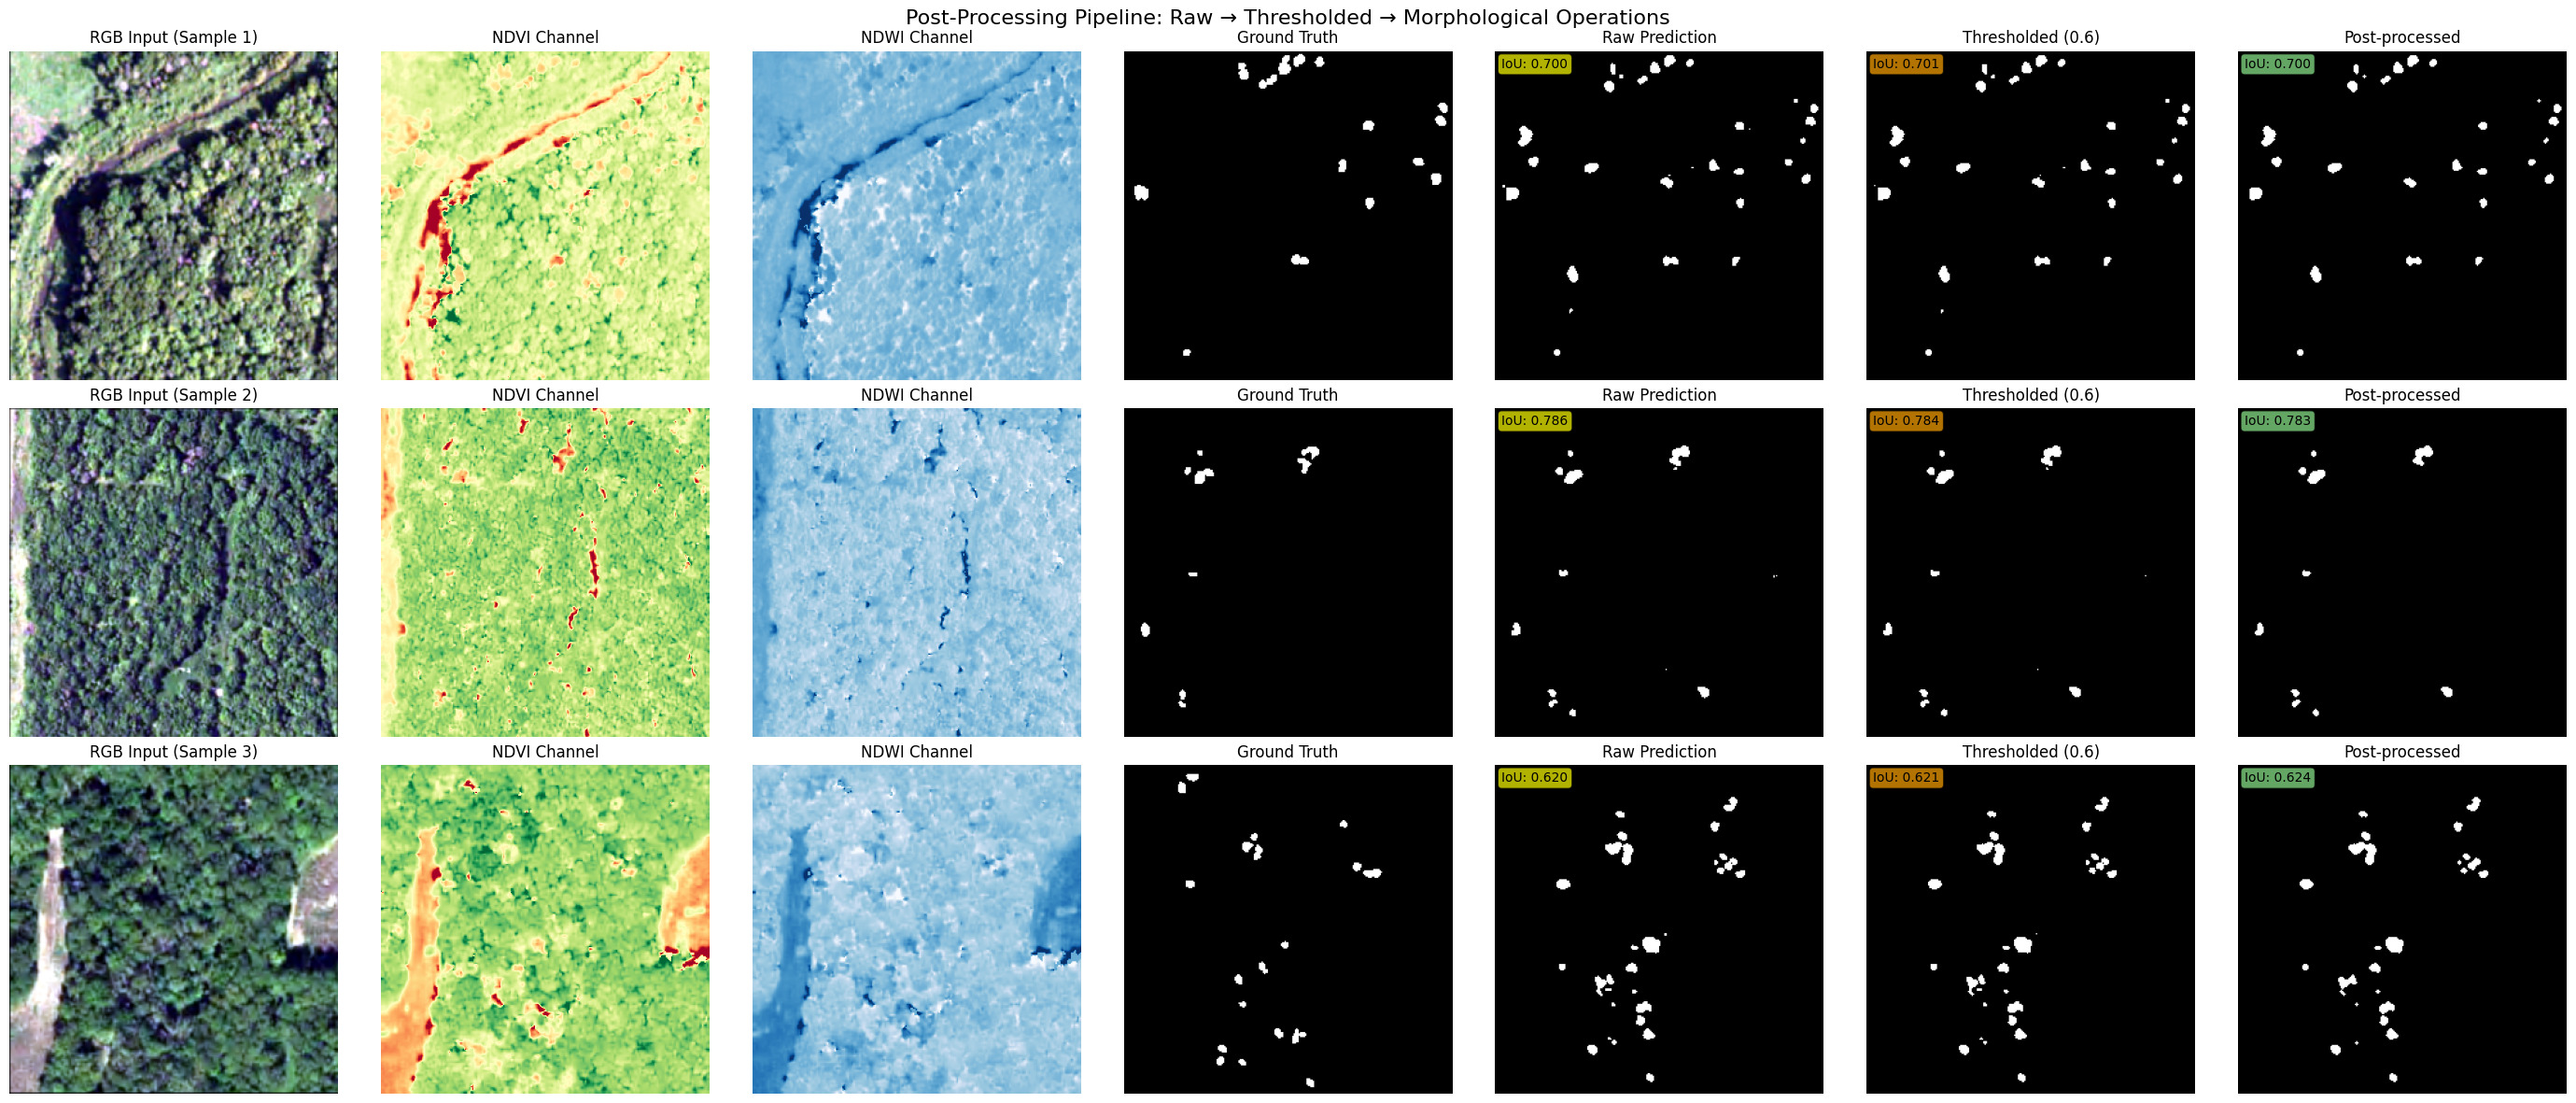
\includegraphics[width=.9\linewidth]{figs/unet-pipeline-compared.jpg}
  \caption{imperfect ablation studies:\\ raw predictions → probability thresholding → morphological cleaning}
  \label{fig:postprocessing}
\end{figure}

\paragraph{Training Configuration.}
The model was trained for 150 epochs using Adam optimiser (lr $= 10^{-3}$) with data augmentation including horizontal/vertical flips and 10° rotations. Input images were resized to $256 \times 256$ with batch size 8. All experiments were conducted on UNSW's Katana high-performance computing cluster\,\cite{b18}. The best model achieved a validation IoU of \textbf{0.7078} after post-processing, representing a significant improvement over the raw prediction IoU of 0.6634.

\newpage
\section{Experimental Results}
Included below are all the experimental results proved by this table.
We report mean Intersection-over-Union (mIoU) on test set.
Intersection-over-Union refers to the total percent of the true mask and the generated mask that overlap, divided by the size of both masks
For DeepLabV3+, the data are split \textbf{80/20} into training, validation.
\begin{table}[h]
  \centering
  \begin{large} 
  \begin{tabular}{|l|r|}
    \hline
    \textbf{Model} & \textbf{IoU} \\ \hline
    UNet           & 0.705  \\ \hline
    CNN            & 0.2862 \\ \hline
    DeepLabV3+ (with CBAM) & 0.4000 \\ \hline
    Random Forest  & 0.1274 \\ \hline
    SGD            & 0.0640 \\ \hline
  \end{tabular}
  \end{large}
\end{table}

\section{Discussion}

\section{Conclusion}

This work demonstrates the superiority of deep encoder-decoder architectures for dead tree segmentation in aerial imagery. Our 8-channel U-Net, leverages multi-spectral inputs (RGB + NRG) with computed vegetation indices (NDVI, NDWI) to achieve an IoU of 0.7078—a 76\% improvement over attention-based alternatives and 146\% over simple CNNs.

Our key findings include: \emph{(i)} spectral feature engineering proves essential, with NDVI/NDWI indices providing another two channels of information on an otherwise small dataset; \emph{(ii)} composite loss functions (Dice + Focal (+ Tversky)) effectively address extreme class imbalance where the traditional BCE proves insufficient; \emph{(iii)} morphological post-processing consistently improves IoU by ~0.04 through noise removal while preserving fragmented tree structures; \emph{(iv)} parameter efficiency analysis reveals that 31M-parameter U-Nets justify their complexity through superior boundary localisation compared to lightweight alternatives.

Classical ML approaches (Random Forest, SGD) fail due to pixel-wise independence assumptions that ignore spatial context. DeepLabV3+ with CBAM, despite sophisticated attention mechanisms, underperforms due to insufficient skip connections for thin structure recovery.

Potential future work could explore:
\emph{(a)} \textbf{Auto-configuration with nnUNet}. The nnUNet framework automatically tunes patch size, learning rate, and augmentation strategy for each dataset; porting our 8-channel input to nnUNet may squeeze out further boundary-level gains without manual hyper-parameter search.  
\emph{(b)} \textbf{HoG, LBP}.  Hand-crafted texture descriptors—Histogram of Oriented Gradients (HoG) and Local Binary Patterns (LBP)—encode bark roughness and canopy granularity that spectral indices alone miss. Concatenating HoG/LBP maps with NDVI/NDWI and feeding them to Random Forests or SVMs may restore spatial awareness, thus producing a best of both worlds, with high-accuracy and light-weight inference.

These extensions would not only tighten IoU on dead-tree masks but also enrich the research on multi-class forest-health monitoring and fine-grained vegetation tasks in general.

\newpage
\section{}


\begin{thebibliography}{00}

% First citation: b20 (dataset) - appears in introduction
\bibitem{b1} M. Ahishali, ``Aerial Imagery for Standing Dead Tree Segmentation,'' Kaggle Datasets, 2025. [Online]. Available: \url{https://www.kaggle.com/datasets/meteahishali/aerial-imagery-for-standing-dead-tree-segmentation}. Accessed: Aug. 9, 2025.

% Second citation: b29 (Stereńczak 2017) - appears in literature review
\bibitem{b2} K. Stereńczak, B. Kraszewski, M. Mielcarek, and Ż. Piasecka, ``Inventory of standing dead trees in the surroundings of communication routes -- The contribution of remote sensing to potential risk assessments,'' \textit{Forest Ecology and Management}, vol. 402, pp. 76--91, 2017.

% Third citation: b25 (Cheng 2024) - appears in literature review  
\bibitem{b3} Y. Cheng et al., ``Scattered tree death contributes to substantial forest loss in California,'' \textit{Nature Communications}, vol. 15, no. 1, 2024.

% Fourth citation: b28 (McRoberts 2007) - appears in literature review
\bibitem{b4} R. E. McRoberts and E. O. Tomppo, ``Remote sensing support for national forest inventories,'' \textit{Remote Sensing of Environment}, vol. 110, no. 4, pp. 412--419, 2007.

% Fifth citation: b27 (Liu 2021) - appears in literature review
\bibitem{b5} X. Liu, J. Frey, M. Denter, K. Zielewska-Büttner, N. Still, and B. Koch, ``Mapping standing dead trees in temperate montane forests using a pixel- and object-based image fusion method and stereo WorldView-3 imagery,'' \textit{Ecological Indicators}, vol. 133, 2021.

% Sixth citation: b24 (Briechle 2021) - appears in literature review
\bibitem{b6} S. Briechle, P. Krzystek, and G. Vosselman, ``Silvi-Net -- A dual-CNN approach for combined classification of tree species and standing dead trees from remote sensing data,'' \textit{International Journal of Applied Earth Observation and Geoinformation}, vol. 98, 2021.

% Seventh citation: b23 (Briechle 2020) - appears in literature review
\bibitem{b7} S. Briechle, P. Krzystek, and G. Vosselman, ``Classification of tree species and standing dead trees by fusing UAV-based LiDAR data and multispectral imagery in the 3D deep neural network PointNet,'' \textit{ISPRS Annals of the Photogrammetry, Remote Sensing and Spatial Information Sciences}, vol. V-2-2020, pp. 203--210, 2020.

% Eighth citation: b18 (Ahishali ADA-Net) - appears in methods section
\bibitem{b8} M. Ahishali, A. U. Rahman, E. Heinaro, and S. Junttila, ``ADA-Net: Attention-Guided Domain Adaptation Network with Contrastive Learning for Standing Dead Tree Segmentation Using Aerial Imagery,'' arXiv preprint arXiv:2504.04271, 2025. [Online]. Available: \url{https://arxiv.org/abs/2504.04271}. Accessed: Aug. 8, 2025.

% Ninth citation: b8 (GeeksforGeeks RF) - appears in methods section
\bibitem{b9} ``Random Forest Algorithm in Machine Learning,'' GeeksforGeeks, Jul. 23, 2025. [Online]. Available: \url{https://www.geeksforgeeks.org/machine-learning/random-forest-algorithm-in-machine-learning/}.

% Tenth citation: b9 (Ganie SGD 2023) - appears in methods section
\bibitem{b10} A. G. Ganie and S. Dadvandipour, ``From big data to smart data: a sample gradient descent approach for machine learning,'' \textit{Journal of Big Data}, vol. 10, no. 1, Oct. 2023. doi: \url{https://doi.org/10.1186/s40537-023-00839-9}.

% Eleventh citation: b10 (Awad SVM 2015) - appears in methods section
\bibitem{b11} M. Awad and R. Khanna, ``Support Vector Machines for Classification,'' in \textit{Efficient Learning Machines}, pp. 39--66, 2015. doi: \url{https://doi.org/10.1007/978-1-4302-5990-9_3}.

% Twelfth citation: b11 (Wilimitis 2018) - appears in methods section
\bibitem{b12} D. Wilimitis, ``The Kernel Trick in Support Vector Classification,'' \textit{Medium}, Dec. 12, 2018. [Online]. Available: \url{https://medium.com/data-science/the-kernel-trick-c98cdbcaeb3f}.

% Thirteenth citation: b1 (Ronneberger U-Net 2015) - appears in U-Net section
\bibitem{b13} O. Ronneberger, P. Fischer, and T. Brox, ``U-Net: Convolutional Networks for Biomedical Image Segmentation,'' in \textit{Medical Image Computing and Computer-Assisted Intervention (MICCAI)}, 2015. [Online]. Available: \url{https://lmb.informatik.uni-freiburg.de/people/ronneber/u-net}.

% Fourteenth citation: b4 (NDVI Wikipedia) - appears in U-Net section
\bibitem{b14} ``Normalized Difference Vegetation Index,'' Wikipedia, Wikimedia Foundation. [Online]. Available: \url{https://en.wikipedia.org/wiki/Normalized_difference_vegetation_index}. Accessed: Jun. 22, 2025.

% Fifteenth citation: b3 (NDWI Wikipedia) - appears in U-Net section
\bibitem{b15} ``Normalized Difference Water Index,'' Wikipedia, Wikimedia Foundation. [Online]. Available: \url{https://en.wikipedia.org/wiki/Normalized_difference_water_index}. Accessed: Apr. 7, 2025.

% Sixteenth citation: b19 (Zagoruyko) - appears in U-Net section
\bibitem{b16} S. Zagoruyko, ``pytorchviz -- Visualizing PyTorch Execution Graphs,'' GitHub. [Online]. Available: \url{https://github.com/szagoruyko/pytorchviz}. Accessed: Aug. 9, 2025.

% Seventeenth citation: b16 (Anthropic Claude) - appears in U-Net section
\bibitem{b17} Anthropic, ``Claude,'' 2023. [Online]. Available: \url{https://www.anthropic.com/claude}. Accessed: Aug. 8, 2025.

% Eighteenth citation: b17 (UNSW Katana) - appears in U-Net section
\bibitem{b18} UNSW Sydney Research Technology Services, ``Katana High-Performance Computing Cluster,'' 2025. [Online]. Available: \url{https://docs.restech.unsw.edu.au/index.html}. Accessed: Aug. 8, 2025.

% Nineteenth citation: b21 (Labml.ai) - appears in U-Net discussion section
\bibitem{b19} Labml.ai, ``U-Net: Annotated PyTorch Implementation.'' [Online]. Available: \url{https://nn.labml.ai/unet/index.html}. Accessed: Aug. 9, 2025.

% Twentieth citation: b22 (Qi Snake Conv) - appears in U-Net discussion section
\bibitem{b20} Y. Qi, Y. He, X. Qi, Y. Zhang, and G. Yang, ``Dynamic Snake Convolution Based on Topological Geometric Constraints for Tubular Structure Segmentation,'' arXiv preprint arXiv:2307.08388, Jul. 17, 2023. [Online]. Available: \url{https://arxiv.org/abs/2307.08388}.

\end{thebibliography}

\end{document}
